\documentclass[a4paper,12pt]{article}

% --- Pacchetti ---
\usepackage[utf8]{inputenc}
\usepackage[italian]{babel}
\usepackage[T1]{fontenc} 
\usepackage{geometry} 
\geometry{margin=2.5cm}
\usepackage{tabularx} % Per tabelle flessibili
\usepackage{booktabs} % Per linee delle tabelle più eleganti
\usepackage{enumitem} % Per personalizzare le liste
\usepackage{graphicx} % Per includere immagini (se necessario)
\usepackage{float} % Per posizionare le figure
\usepackage{amsmath} % Per formule matematiche
\usepackage{listings}
\usepackage{xcolor}

% Configurazione per il codice SQL
\lstset{
    language=SQL,
    basicstyle=\ttfamily\small,
    keywordstyle=\color{blue}\bfseries,
    commentstyle=\color{gray},
    stringstyle=\color{green!50!black},
    breaklines=true,
    postbreak=\mbox{\textcolor{red}{$\hookrightarrow$}\space},
    frame=single,
    showstringspaces=false,
    morekeywords={HAVING,COUNT,DISTINCT,EXISTS}
}
\title{Progetto di Basi di Dati}
\author{Federico Del Pup \\ Luigi Pa\textcommabelow{s}cu \\ Matteo Passador \\ Stefano Toneguzzo}
\date{\today}

\begin{document}

\maketitle
\section{Indice}
\begin{itemize}
    \item \textbf{Glossario dei termini} (Sezione 2)
    \item \textbf{Strutturazione dei requisiti} (Sezione 3)
    \item \textbf{Tavola dei volumi} (Sezione 4)
    \item \textbf{Schema concettuale} (Sezione 5)
    \item \textbf{Schema logico} (Sezione 6)
    \item \textbf{Operazioni e Query} (Sezione 7)
    \item \textbf{Trigger} (Sezione 8)
\end{itemize}

\section{Analisi dei requisiti}
\subsection{Introduzione alla richiesta}
Il progetto richiede la progettazione di una base di dati relazionale per la gestione di una bibliografia, con un focus specifico sulle pubblicazioni accademiche. La base di dati deve essere in grado di gestire un ampio insieme di pubblicazioni, ciascuna caratterizzata da attributi specifici e relazioni complesse con autori, affiliazioni, editori, ecc. L'obiettivo è creare un modello concettuale che rappresenti fedelmente il dominio, seguito da una progettazione logica e fisica che ottimizzi le operazioni più frequenti, come la stampa dei dati e l'inserimento di nuove pubblicazioni. Inoltre, è richiesta l'implementazione di trigger per mantenere l'integrità dei dati e l'efficienza delle query, nonché la definizione di operazioni e query specifiche per l'analisi dei dati bibliografici.
\subsection{Glossario dei termini}

\begin{tabularx}{\textwidth}{l X X}
\toprule
\textbf{Termine} & \textbf{Descrizione} & \textbf{Collegamenti} \\
\midrule
Pubblicazione & Elemento di bibliografia & Autore, Pubblicazione \\
Articolo su rivista & Tipo di pubblicazione & Autore, Pubblicazione \\
Articolo per conferenza & Tipo di pubblicazione & Autore, Pubblicazione \\
Libro & Tipo di pubblicazione & Autore, Pubblicazione, Editor \\
Tesi & Tipo di pubblicazione & Autore, Pubblicazione, Università \\
Autore & Persona che scrive una pubblicazione & Pubblicazione, Affiliazione \\
Affiliazione & Gruppo di autori & Autore \\
Editore & Entità che pubblica un libro & Libro \\
Università & Luogo di discussione della tesi & Tesi \\
\bottomrule
\end{tabularx}

\subsection{Strutturazione dei requisiti}

\subsubsection{Frasi di carattere generale}
Si supponga di aver collezionato il seguente insieme di requisiti per la progettazione di una base di dati relazionale per la gestione di una bibliografia. Una bibliografia è costituita da un insieme di pubblicazioni.

\subsubsection{Dettaglio dei requisiti}
\begin{itemize}[label=\textbullet]
    \item \textbf{Pubblicazioni:} Ogni pubblicazione è caratterizzata da un codice univoco, un titolo, un anno di pubblicazione e uno o più autori. È presente una lista di riferimenti bibliografici (citazioni) verso altre pubblicazioni della bibliografia. Ogni pubblicazione tiene traccia del numero di citazioni ricevute.
    
    \item \textbf{Articoli su rivista:} Si registrano il nome della rivista, il numero del volume, le pagine (iniziale e finale) e il numero totale di pagine.
    
    \item \textbf{Articoli per conferenza:} Si registrano nome e luogo della conferenza, anno di svolgimento (indipendente dall'anno di pubblicazione), pagine (iniziale/finale) e totale pagine.
    
    \item \textbf{Libri:} Identificati dal codice ISBN, includono l'editore e il numero totale di pagine.
    
    \item \textbf{Tesi:} Si memorizzano l'argomento, l'università di discussione e il numero totale di pagine.
    
    \item \textbf{Autori:} Di ogni autore si memorizzano nome, cognome, email, pagina Web e una o più affiliazioni.
    
    \item \textbf{Affiliazioni:} Descritte da nome, indirizzo completo (via, civico, città, nazione) e numero di telefono.
    
    \item \textbf{Editori:} Descritti da nome e indirizzo fisico.
    
    \item \textbf{Università:} Identificate univocamente dal nome, includono indirizzo e telefono.
\end{itemize}

\section{Progettazione concettuale}
\subsection{Gestione dell'entità Pubblicazione e delle sue specializzazioni}
\subsection{Gestione dell'entità Affiliazione e delle sue specializzazioni}
\subsection{Gestione della relazione Tesi-Affiliazione e di Autore}
\begin{figure}[H]
    \centering
    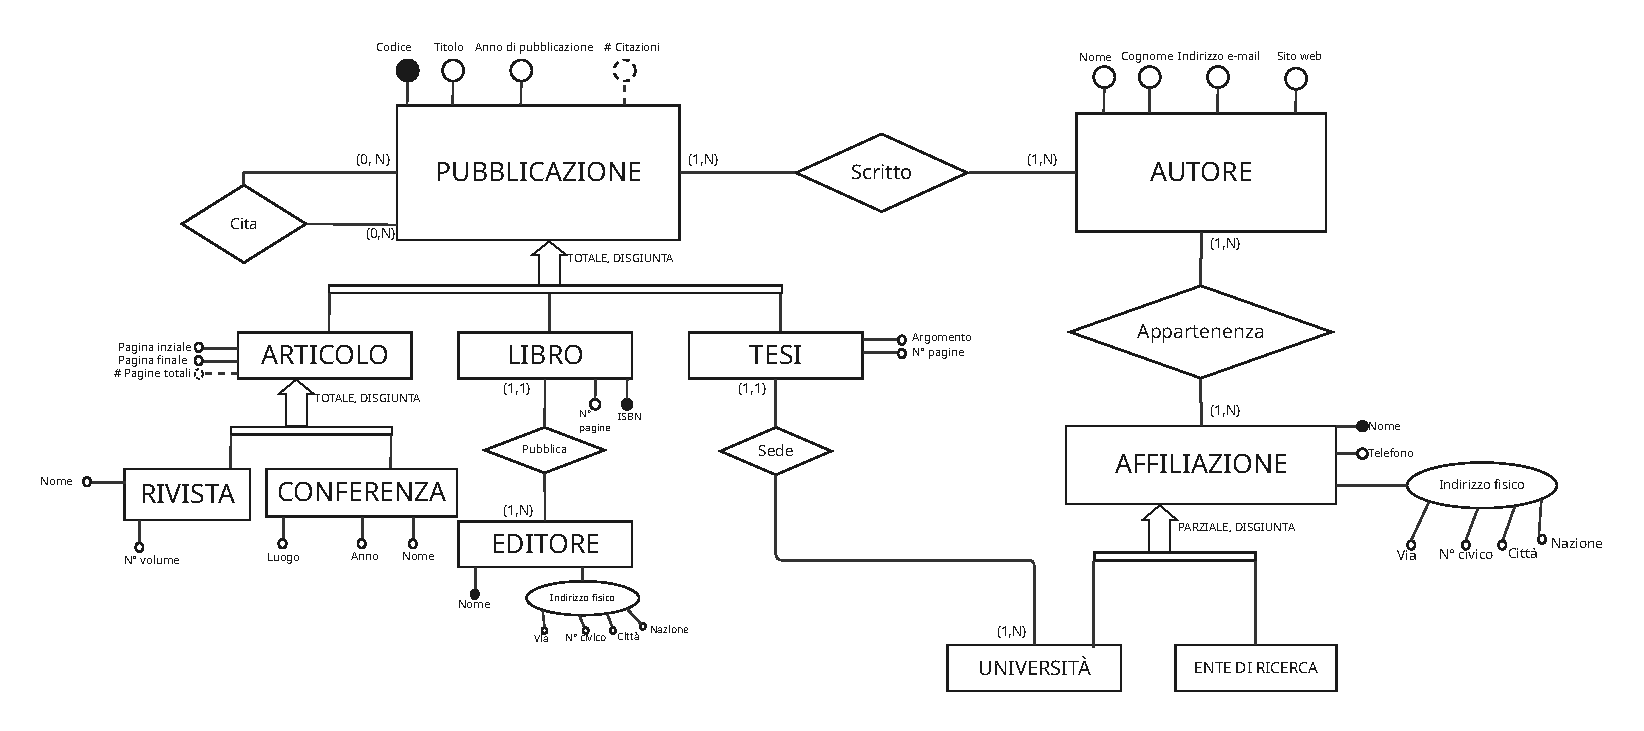
\includegraphics[width=0.8\textwidth]{img/SchemaER.pdf} % image file path
    \caption{Schema Entità-Relazione}
    \label{fig:label_immagine}
\end{figure}

\section{Progettazione logica}
\subsection{Tavola dei volumi}

\begin{tabularx}{\textwidth}{l c r}
\toprule
\textbf{Concetto} & \textbf{Tipo} & \textbf{Volume} \\
\midrule
Pubblicazione & E & 100.000 \\
Articolo su rivista & E & 20.000 \\
Articolo per conferenza & E & 15.000 \\
Libro & E & 10.000 \\
Tesi & E & 55.000 \\
Autore & E & 70.000 \\
Affiliazione & E & 500 \\
Editore & E & 400 \\
Università & E & 300 \\
Ente di ricerca & E & 200 \\
\midrule
Citazione & R & $100.000 \times 20$ \\
Scritto & R & $3,3 \times 100.000$ \\
Appartenenza & R & $70.000 \times 2$ \\
Sede & R & 55.000 \\
Pubblica & R & 10.000 \\
\bottomrule
\end{tabularx}

\medskip

La tavola dei volumi rappresenta il passaggio fondamentale dalla progettazione concettuale a quella logica, fornendo una stima quantitativa del carico che il database dovrà sostenere. Il sistema gestisce un totale di \textbf{100.000 pubblicazioni}. Si noti come la somma delle entità figlie (\textit{Articolo su rivista, Articolo per conferenza, Libro, Tesi}) sia esattamente pari a 100.000, riflettendo la scelta di una \textbf{gerarchia a copertura totale}. Le tesi rappresentano la quota maggioritaria (55.000), coerentemente con un dominio accademico.

La relazione \texttt{Citazione} è la più onerosa del sistema, con un volume stimato di \textbf{2.000.000 di record} ($100.000 \times 20$). Questa dimensione giustifica l'introduzione dell'attributo derivato \texttt{NumeroCitazioni} per ottimizzare le operazioni di sola lettura, nonostante l'aggravio nei tempi di inserimento. In seguito viene mostrata un'analisi comparativa tra le due soluzioni, evidenziando i trade-off in termini di costo computazionale per le operazioni più frequenti.
Con \textbf{70.000 autori} e una media di 3,3 autori per pubblicazione (relazione \texttt{Scritto}), il sistema deve gestire circa 330.000 legami autore-opera. La relazione \texttt{Appartenenza} ($70.000 \times 2$) modella correttamente il turnover accademico, prevedendo che ogni autore sia mediamente affiliato a due enti diversi nel tempo.
Il numero contenuto di \textbf{Affiliazioni (500)}, \textbf{Editori (400)} e \textbf{Università (300)} suggerisce che queste tabelle fungeranno da "anagrafiche di controllo", con un basso tasso di aggiornamento rispetto alle tabelle transazionali delle pubblicazioni e citazioni.
\subsection{Analisi delle ridondanze}
\subsubsection*{Frequenza delle Operazioni più comuni}
Ecco una stima della frequenza delle operazioni più comuni che il sistema dovrà gestire, basata su ipotesi ragionevoli e coerenti con il dominio accademico:
\begin{enumerate}[label=\textbf{OP\arabic*}, start=1, leftmargin=1.5cm]
    \item \textbf{Stampa delle pubblicazioni} \\
    Frequenza: 200/500 volte al giorno.
    
    \item \textbf{Inserimento e Aggiornamento} \\
    Inserire una pubblicazione (40 volte al giorno). \\
    Aggiornamento delle citazioni di una pubblicazione (40 volte al giorno)

    \item \textbf{Inserire un autore} \\
    Frequenza: 10 volte al giorno.

    \item \textbf{Modifica autore/affiliazione} \\
    Frequenza: 1 volta al giorno (frequenza stimata).
\end{enumerate}
Gli unici due attributi ridondanti presenti nello schema sono: \texttt{NumeroCitazioni} nell'entità \textbf{Pubblicazione} e \texttt{NumeroPagineTotali} nell'entità \textbf{Articolo}. Il primo è stato introdotto per ottimizzare le operazioni di stampa dei dati generali (\textit{OP1}). Il secondo è superfluo, in quanto è possibile calcolarlo dinamicamente come differenza tra \texttt{PaginaFinale} e \texttt{PaginaIniziale} più uno. Di seguito viene mostrata un'analisi comparativa tra le due soluzioni per la prima ridondanza, evidenziando i trade-off in termini di costo computazionale per le operazioni più frequenti.

\subsubsection{Con Ridondanza dell'attributo NumeroCitazioni}
*Nota: Per il calcolo del costo, si assume che un accesso a un'entità o relazione di tipo "L" (lettura) abbia un costo unitario di 1, mentre un accesso di tipo "S" (scrittura) abbia un costo unitario di 2, riflettendo l'overhead aggiuntivo associato alle operazioni di scrittura rispetto a quelle di lettura. 
La stima del costo totale è effettuata con il dato di frequenza maggiore per ogni operazione, al fine di valutare l'impatto massimo della ridondanza sull'efficienza del sistema.
\subsubsection*{Operazione 1}
\begin{tabular}{llll}
\toprule
\textbf{Concetto} & \textbf{Costrutto} & \textbf{Accessi} & \textbf{Tipo} \\
\midrule
Pubblicazione & Entità & 1 & L \\
\bottomrule
\end{tabular}

\medskip
\textbf{Costo:} $(500 \times 1) \times 1 = 500$ unità di costo

\subsubsection*{Operazione 2}
\begin{tabular}{llll}
\toprule
\textbf{Concetto} & \textbf{Costrutto} & \textbf{Accessi} & \textbf{Tipo} \\
\midrule
Pubblicazione & Entità & 2 & S \\
Cita          & Relazione & 1 & S \\
Pubblicazione & Entità & 1 & L \\
Autore        & Entità & 1 & S \\
\bottomrule
\end{tabular}

\paragraph{Passi logici:}
\begin{enumerate}[label=\textbf{\arabic*)}, start=1, leftmargin=1.5cm]
    \item Salvo i dati della pubblicazione
    \item Salvo le coppie di pubblicazione e pubblicazione citata
    \item Cerco la pubblicazione citata
    \item Incremento di 1 il numero di citazioni a quella pubblicazione
    \item Salvo la coppia pubblicazione autore
\end{enumerate}

\textbf{Costo:} $(40 \times 4) \times 2 + (40 \times 1) \times 1 = 360$ unità

\subsubsection{Senza Ridondanza dell'attributo NumeroCitazioni}

\subsubsection*{Operazione 1}
\begin{tabular}{llll}
\toprule
\textbf{Concetto} & \textbf{Costrutto} & \textbf{Accessi} & \textbf{Tipo} \\
\midrule
Pubblicazione & Entità    & 1  & L \\
Citazione     & Relazione & 20 & L \\
\bottomrule
\end{tabular}

\paragraph{Descrizione:} 
Stampo i dati relativi ad una pubblicazione. Per ogni pubblicazione, per calcolare il numero di citazioni dobbiamo accedere in media alla relazione ``citazione'', calcolato come: $\frac{\text{volume Citazione}}{\text{volume Pubblicazioni}} = 20$.

\medskip
\textbf{Costo:} $500 \times (20 + 1) \times 1 = 10.500$ unità di costo

\subsubsection*{Operazione 2}
\begin{tabular}{llll}
\toprule
\textbf{Concetto} & \textbf{Costrutto} & \textbf{Accessi} & \textbf{Tipo} \\
\midrule
Pubblicazione & Entità & 1 & S \\
Cita          & Relazione & 1 & S \\
Autore        & Entità & 1 & S \\
\bottomrule
\end{tabular}

\paragraph{Passi logici:}
\begin{enumerate}[label=\textbf{\arabic*)}, start=1, leftmargin=1.5cm]
    \item Salvo i dati della pubblicazione
    \item Salvo le coppie di pubblicazione e pubblicazione citata
    \item Salvo la coppia pubblicazione autore
\end{enumerate}

\medskip
\textbf{Costo:} $40 \times 3 \times 2 = 240$ unità di costo

\subsubsection{Studio Comparativo}

\begin{table}[h]
\centering
\begin{tabular}{lcc}
\toprule
\textbf{Costo} & \textbf{Presenza di ridondanza} & \textbf{Assenza di ridondanza} \\
\midrule
OP1 & 500 & 10.500 \\
OP2 & 360 & 240 \\
\midrule
\textbf{Totale} & \textbf{860} & \textbf{10.740} \\
\bottomrule
\end{tabular}
\end{table}

\textbf{Conclusione:} Poiché $860 < 10.740$, conviene mantenere l'attributo derivato.

\subsection{Ristrutturazione dello schema ER}
\begin{figure}[H]
    \centering
    \includegraphics[width=0.8\textwidth]{img/SchemaERpt1.pdf} % image file path
    \caption{Schema ER modificato dopo la prima revisione}
    \label{fig:label_immagine2}
\end{figure}
\noindent
\textbf{Specializzazione Rivista-Conferenza:} 
La gerarchia è stata accorpata verso l'alto (ristrutturazione verso il padre) eliminando le entità figlie e migrandone gli attributi nell'entità genitore \textit{Articolo}. Per distinguere le occorrenze, è stato introdotto l'attributo discriminante \textit{Tipo}, i cui valori sono vincolati al dominio $\{\text{Rivista, Conferenza}\}$. 

Gli attributi derivanti dalle classi figlie sono stati definiti come opzionali (cardinalità 0..1), con l'eccezione dell'attributo \textit{Nome}, che rimane obbligatorio in quanto comune a entrambe le tipologie. Si specifica, inoltre, che l'attributo \textit{AnnoConferenza} deve essere semanticamente distinto dall'attributo \textit{AnnoPubblicazione}.

\begin{figure}[H]
    \centering
    \includegraphics[width=0.8\textwidth]{img/SchemaERpt2.pdf} % image file path
    \caption{Schema ER modificato dopo la seconda revisione}
    \label{fig:label_immagine3}
\end{figure}

\noindent
\textbf{Semplificazione della Gerarchia Affiliazione:}
La specializzazione tra l'entità \textit{Affiliazione} (padre) e le sottoclassi \textit{Università} ed \textit{Ente di Ricerca} è stata risolta mediante l'accorpamento verso il padre. Tale scelta è motivata dall'assenza di attributi specifici rilevanti nelle entità figlie. 

Per preservare la semantica originale, è stato introdotto un vincolo di integrità basato sul tipo di affiliazione: l'associazione con l'entità \textit{Tesi} è valida esclusivamente per le occorrenze di tipo \textit{Università}. In termini di cardinalità, il rapporto tra \textit{Tesi} ed \textit{Affiliazione} è di $(1,1)$, mentre la partecipazione dell'entità \textit{Affiliazione} è $(0,n)$, poiché solo il sottoinsieme relativo alle università può essere associato a una tesi.

\noindent
\textbf{Semplificazione dell'attributo Indirizzo:}
L'attributo composto \textit{Indirizzo Fisico} è stato ristrutturato mediante un processo di aggregazione dei suoi componenti (quali via, numero civico, CAP e città). Al fine di semplificare l'implementazione nel modello logico e facilitare le operazioni di inserimento, i singoli campi sono stati unificati in un unico attributo atomico di tipo stringa.


\begin{figure}[H]
    \centering
    \includegraphics[width=0.8\textwidth]{img/SchemaERpt3.pdf} % image file path
    \caption{Schema ER modificato dopo la terza revisione}
    \label{fig:label_immagine4}
\end{figure}

\noindent
\textbf{Risoluzione della Gerarchia Pubblicazione:}
La specializzazione tra l'entità genitore \textit{Pubblicazione} e le sottoclassi \textit{Articolo}, \textit{Libro} e \textit{Tesi} è stata risolta mantenendo le entità distinte (strategia delle entità multiple). 

Per implementare correttamente il legame logico, sono state definite relazioni esplicite tra il padre e i figli tramite l'uso di chiavi esterne (\textit{foreign keys}) nelle entità figlie che referenziano la chiave primaria di \textit{Pubblicazione}. Al fine di garantire la copertura totale della specializzazione, è stato introdotto un vincolo di integrità aggiuntivo: ogni occorrenza dell'entità \textit{Pubblicazione} deve necessariamente essere referenziata come chiave esterna in almeno una delle tre entità figlie.

\begin{figure}[H]
    \centering
    \includegraphics[width=0.8\textwidth]{img/SchemaERpt4.pdf} % image file path
    \caption{Schema ER modificato dopo la quarta revisione}
    \label{fig:label_immagine5}
\end{figure}


\noindent
\textbf{Ristrutturazione della relazione "Scritto" e "Appartenenza":}
La relazione \textit{Scritto} è stata ristrutturata in modo da inserire un'entità associativa, denominata \textit{Pubb-Autori}, che collega l'entità \textit{Autore} con l'entità \textit{Pubblicazione}. Questa scelta è motivata dalla necessità di rappresentare correttamente la relazione molti-a-molti tra autori e pubblicazioni, consentendo di gestire efficacemente i casi in cui una pubblicazione abbia più autori e un autore abbia più pubblicazioni. Lo stesso approccio è stato adottato per la relazione \textit{Appartenenza}, con l'introduzione dell'entità associativa \textit{Aut-Aff} che collega l'entità \textit{Autore} con l'entità \textit{Affiliazione}. Questa ristrutturazione consente di modellare in modo più flessibile le dinamiche di affiliazione degli autori, che possono essere associati a più enti nel tempo, e di mantenere una chiara tracciabilità delle relazioni tra autori e affiliazioni.
\begin{figure}[h]
    \centering
    \includegraphics[width=0.8\textwidth]{img/SchemaERfinale.pdf} % image file path
    \caption{Schema ER finale senza le modifiche di dettaglio}
    \label{fig:label_immagine}
\end{figure}


\subsection{Schema logico}

Dal moodello ER finale, si ottiene lo schema logico relazionale seguente:
\\PUBBLICAZIONI(\underline{Codice},Titolo, Anno, NumeroCitazioni) \\
ARTICOLI(\underline{CodicePubblicazione}, Nome, NumeroRivista, LuogoRivista, Anno, PaginaIniziale, PaginaFinale, Tipo) \\
LIBRI(\underline{CodicePubblicazione}, ISBN, NumeroPagine, NomeEditore) \\
TESI(\underline{CodicePubblicazione}, Argomento, NumeroPagine, Affiliazione) \\
AUTORI(\underline{ID}, Nome, Cognome, Email, SitoWeb) \\
AFFILIAZIONI(\underline{Nome}, IndirizzoFisico, NumeroTelefono, Tipo) \\
EDITORI(\underline{Nome}, Indirizzo) \\
CITAZIONI(\underline{PubblicazioneChiamante}, \underline{PubblicazioneCitata}) \\
PUBB-AUTORI(\underline{IDAutore}, \underline{CodicePubblicazione}) \\
AUT-AFF(\underline{IDAutore}, \underline{NomeAffiliazione}) \\
*le chiavi primarie sono sottolineate, mentre le chiavi esterne sono indicate con frecce.
\textbf{Chiavi esterne:} \\
$\text{ARTICOLI.CodicePubblicazione} \rightarrow \text{PUBBLICAZIONI.Codice}$ \\
$\text{LIBRI.CodicePubblicazione} \rightarrow \text{PUBBLICAZIONI.Codice}$ \\
$\text{TESI.CodicePubblicazione} \rightarrow \text{PUBBLICAZIONI.Codice}$ \\
$\text{CITAZIONI.PubblicazioneChiamante} \rightarrow \text{PUBBLICAZIONI.Codice}$ \\
$\text{CITAZIONI.PubblicazioneCitata} \rightarrow \text{PUBBLICAZIONI.Codice}$ \\
$\text{LIBRI.NomeEditore} \rightarrow \text{EDITORI.Nome}$ \\
$\text{TESI.Affiliazione} \rightarrow \text{AFFILIAZIONI.Nome}$ \\
$\text{PUBB-AUTORI.IDAutore} \rightarrow \text{AUTORI.ID}$ \\
$\text{PUBB-AUTORI.CodicePubblicazione} \rightarrow \text{PUBBLICAZIONI.Codice}$ \\
$\text{AUT-AFF.IDAutore} \rightarrow \text{AUTORI.ID}$ \\
$\text{AUT-AFF.NomeAffiliazione} \rightarrow \text{AFFILIAZIONI.Nome}$ \\
\\
Si noti che le chiavi primarie sono state definite in modo da garantire l'univocità di ogni record, mentre le chiavi esterne sono state implementate per mantenere l'integrità referenziale tra le tabelle, assicurando che le relazioni logiche tra i dati siano rispettate. L'unica chiave candidabile non scelta come chiave primaria è l'ISBN nella tabella \textbf{LIBRI}, poiché il codice della pubblicazione è già un identificatore univoco sufficiente per distinguere ogni libro all'interno del sistema. Si è preferito mantenere un'unica chiave primaria per semplificare le operazioni di join e ridurre la complessità del modello, evitando la necessità di gestire chiavi composite o multiple per la stessa entità. \\


\section{Progettazione fisica (Implementazione DB)}

\subsection{Generazione delle tabelle SQL}


\subsection{Popolamento del database}

\subsection{Trigger}
\subsubsection*{Trigger per l'aggiornamento del numero di citazioni}
\textbf{Non Autocitazione}: Una pubblicazione non può citare sé stessa. Questo è il vincolo più elementare e serve a prevenire l'inserimento di dati logicamente inconsistenti, garantendo che il conteggio delle citazioni rifletta solo i riferimenti esterni.\\
\textbf{Non Citazione Circolare}: Una pubblicazione A non può citare una pubblicazione B se B cita già A, direttamente o indirettamente. Questo vincolo impedisce la formazione di cicli di citazione che potrebbero distorcere il conteggio delle citazioni e complicare l'analisi bibliometrica.\\
\textbf{Nota sul Vincolo Temporale}: Una pubblicazione non può citare un'altra pubblicazione con un anno di pubblicazione successivo. Pur riconoscendo l'esistenza di casi come i preprint nel mondo reale, per coerenza logica del modello e per semplicità, questo vincolo è assunto come rilevante e implementato nel database.\\

\section{Query}

\begin{enumerate}[label=\textbf{OP\arabic*}, start=5, leftmargin=1.5cm]
    \item \textbf{Autore con più pubblicazioni per affiliazione} \\
    Stampare il nome dell'autore che detiene il maggior numero di pubblicazioni per ogni singola affiliazione.
    
    \item \textbf{Co-autoria esclusiva} \\
    Stampare le coppie di autori che hanno collaborato sempre e solo tra di loro (ovvero, ogni loro pubblicazione è stata fatta in coppia).
    
    \item \textbf{Autori fedeli all'affiliazione} \\
    Stampare gli autori che non hanno mai prodotto pubblicazioni con co-autori appartenenti a un'affiliazione diversa dalla propria.
    
    \item \textbf{Analisi dell'impatto a breve termine} \\
    Trovare gli autori che hanno pubblicato esclusivamente articoli i quali, a distanza di 2 anni dalla data di pubblicazione, hanno accumulato almeno 5 citazioni.
\end{enumerate}

\subsection*{OP5: Autore con più pubblicazioni per ogni affiliazione}
\begin{lstlisting}
SELECT a.nome, a.cognome, aa.nome_affiliazione
FROM AUTORE a
JOIN PUBB_AUTORE pa ON a.id = pa.id_autore
JOIN AUTO_AFF aa ON a.id = aa.id_autore
GROUP BY a.id, a.nome, a.cognome, aa.nome_affiliazione
HAVING COUNT(pa.codice_pubblicazione) = (
    SELECT MAX(cnt)
    FROM (
        SELECT COUNT(pa2.codice_pubblicazione) AS cnt
        FROM AUTORE a2
        JOIN PUBB_AUTORE pa2 ON a2.id = pa2.id_autore
        JOIN AUTO_AFF aa2 ON a2.id = aa2.id_autore
        WHERE aa2.nome_affiliazione = aa.nome_affiliazione
        GROUP BY a2.id
    ) sub
);
\end{lstlisting}

\subsection*{OP6: Coppie che hanno pubblicato sempre e solo insieme}
\begin{lstlisting}
SELECT pa1.id_autore, pa2.id_autore
FROM PUBB_AUTORE pa1
JOIN PUBB_AUTORE pa2 
    ON pa1.codice_pubblicazione = pa2.codice_pubblicazione 
    AND pa1.id_autore < pa2.id_autore
GROUP BY pa1.id_autore, pa2.id_autore
HAVING COUNT(DISTINCT pa1.codice_pubblicazione) = (
    SELECT COUNT(*) 
    FROM PUBB_AUTORE pa
    WHERE pa.id_autore = pa1.id_autore
)
AND COUNT(DISTINCT pa2.codice_pubblicazione) = (
    SELECT COUNT(*) 
    FROM PUBB_AUTORE pa
    WHERE pa.id_autore = pa2.id_autore
);
\end{lstlisting}

\newpage

\subsection*{OP7: Autori che non hanno mai pubblicato con colleghi di altre affiliazioni}
\textit{Un autore è valido se NON esiste nessuna pubblicazione in cui ha collaborato con un autore di affiliazione diversa.}
\begin{lstlisting}
SELECT a.id, a.nome, a.cognome
FROM AUTORE a
WHERE NOT EXISTS (
    SELECT 1
    FROM PUBB_AUTORE pa1
    JOIN PUBB_AUTORE pa2
        ON pa1.codice_pubblicazione = pa2.codice_pubblicazione
        AND pa1.id_autore <> pa2.id_autore
    JOIN AUTO_AFF aa1
        ON aa1.id_autore = pa1.id_autore
    JOIN AUTO_AFF aa2
        ON aa2.id_autore = pa2.id_autore
    WHERE pa1.id_autore = a.id
      AND aa1.nome_affiliazione <> aa2.nome_affiliazione
);
\end{lstlisting}

\subsection*{OP8: Autori con solo articoli di successo (min. 5 citazioni a 2 anni)}
\begin{lstlisting}
SELECT a.id, a.nome, a.cognome
FROM public.autore a
-- Condizione A: L'autore deve aver pubblicato almeno un articolo
WHERE EXISTS (
    SELECT 1 FROM public.pubb_autore pa WHERE pa.id_autore = a.id
)
-- Condizione B: NON deve esistere alcuna sua pubblicazione "flop"
AND NOT EXISTS (
    SELECT 1
    FROM public.pubb_autore pa
    JOIN public.pubblicazione p ON pa.codice_pubblicazione = p.codice
    WHERE pa.id_autore = a.id
      AND (
          SELECT COUNT(*)
          FROM public.citazione c
          JOIN public.pubblicazione pc ON c.codice_pubblicazione_citante = pc.codice
          WHERE c.codice_pubblicazione_citata = p.codice
            AND (pc.annopubblicazione - p.annopubblicazione) <= 2
      ) < 5
);
\end{lstlisting}

\paragraph{Nota sull'inefficacia dell'attributo derivato nella query OP8:}
Nonostante la presenza dell'attributo derivato \texttt{NumeroCitazioni} nell'entità \textbf{PUBBLICAZIONE} --- introdotto per ottimizzare la stampa dei dati generali (\textit{OP1}) --- esso risulta inutilizzabile ai fini della query \textbf{OP8} (\textit{Analisi dell'impatto a breve termine}).

Il limite risiede nella natura stessa dell'attributo ridondante:
\begin{itemize}
    \item \textbf{Staticità del dato:} L'attributo memorizza esclusivamente il conteggio totale e cumulativo delle citazioni ricevute fino all'istante attuale.
    \item \textbf{Vincolo Temporale Dinamico:} La specifica della \textit{OP8} richiede il filtraggio delle sole citazioni avvenute entro un arco temporale di \textbf{due anni} dalla data di rilascio della pubblicazione.
\end{itemize}

Di conseguenza, per soddisfare il requisito, è necessario ignorare il valore pre-calcolato ed effettuare un calcolo dinamico accedendo direttamente alla relazione \texttt{CITAZIONI}. Questo processo permette di confrontare gli attributi \texttt{Anno} della pubblicazione citante e di quella citata, operazione indispensabile per isolare il sottoinsieme di riferimenti bibliografici pertinenti all'analisi richiesta.

\end{document}